\section{Discussion \& Related Work}
\label{sec:discussion}

Many large-scale benchmarks have been developed to test the general capabilities of frontier LMs, including the Chatbot Arena~\citep{chiang2024chatbot} or LiveBench~\citep{white2025livebench}.
Other benchmarks, such as FrontierMath~\citep{glazer2024frontiermath}, TaskBench~\citep{shen2024taskbench}, GameBench~\citep{costarelli2024gamebench}, and Atari-GPT~\citep{waytowich2024atari}, specifically investigate the reasoning or interactive decision-making capabilities of (L)LMs.
Most closely related to our work, and published in parallel, the BALROG~\citep{paglieri2025balrog} benchmark evaluates frontier LMs' zero-shot reasoning on multimodal decision-making tasks in five game environments from Baby AI to NetHack.
Our work complements these benchmarks by focusing on in-context imitation learning with long multimodal context, filling a gap in the current literature. 
Our benchmark is currently in its ``easiest'' form (\eg grid world without obstacles) and can easily be made more challenging.

\ificlr
\begin{wrapfigure}{r}{0.5\textwidth}
    \vspace{-20pt}
\else
\begin{figure}
\fi
   \begin{center}
        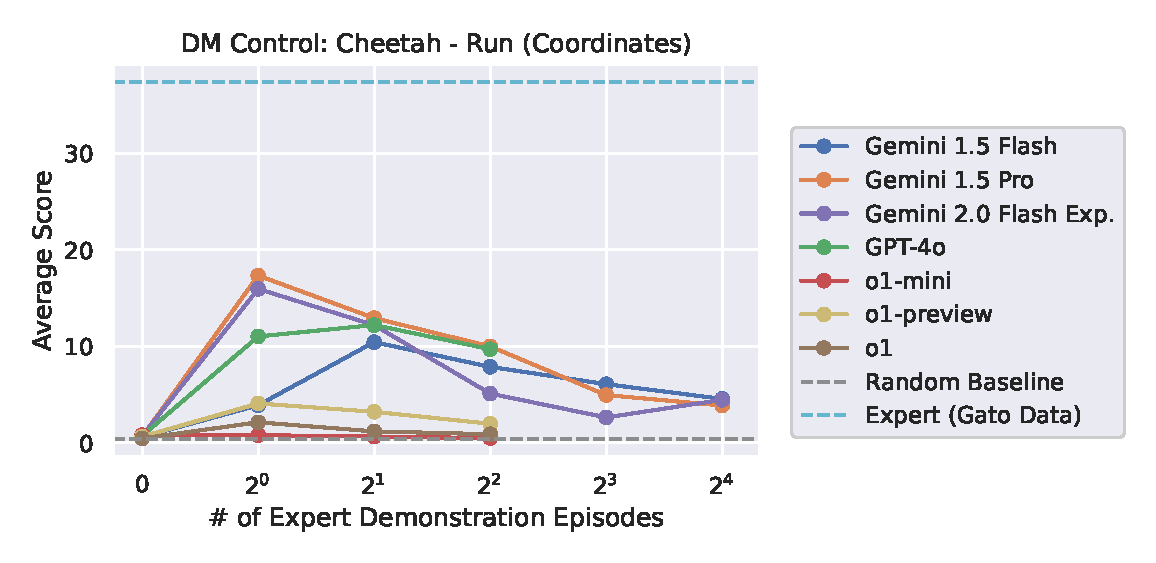
\includegraphics[width=0.5\textwidth]{figures/dm_control_cheetah_run_dict.eps}
    \end{center}
    \vspace{-8pt}
    \caption{
        In-context imitation learning on the cheetah run task from the DM Control suite using position/velocity vector observations encoded as text.
        \pro{} and \expflash{} perform best with a single demonstration episode, \gpt{} and \flash{} with two demonstration episodes, with more demonstrations degrading performance.
        \pro{} achieves the highest performance, roughly half the expert score.
    }
    \label{fig:dm-control}
\ificlr
\end{wrapfigure}
\else
\end{figure}
\fi
There are a few reasons to be optimistic about in-context imitation learning with long-context models.
Many demonstrations should, in principle, improve performance over few-shot learning (as shown by \citet{agarwal2024many, jiang2024many} on non-interactive tasks), and modern LMs have long enough contexts to test this at scale.
Additionally, pretrained LMs have a fairly general ability to recognize and imitate algorithmic patterns in their context \citep{mirchandani2023large}, which is in line with the memory-based meta-learning view on (universal) in-context prediction~\citep{ortega2019meta, grau2024learning}.
If universal enough, models would, with enough observations, recognize and correctly continue environment-agent interaction patterns.
\ificlr
We refer interested readers to \cref{app:related-work} for a more detailed discussion of additional related work.
\else
See \cref{app:related-work} for a discussion of additional related work.
\fi

While we find some cases of steady in-context learning, in the majority of cases LMs' performance is largely independent of the number of demonstrations. 
It is unclear whether in-context imitation learning is not well suited to communicate desired agentic behavior (\ie models do not ``understand'' the task purely from demonstrations), or whether models have difficulty to effectively use a dense long context.
To provide additional insight we perform a ``replay'' control experiment, where a single episode is shown in context, and the same exact episode is evaluated, such that models only need to ``copy'' actions from the demonstration episode.
We find that models (except \mini{}) perform well in this control experiment on all tasks (see \cref{app:additional-results:replay}).

\vspace{-8pt}
\paragraph{Limitations}

We perform an evaluation via closed-source APIs and thus have little control over how the data is processed and fed to the underlying models.
Since models behind the APIs can be updated at any time, it is possible that our results may not be quantitatively reproducible soon after publishing this manuscript.
Despite our best efforts in evaluating different prompt formats, we cannot rule out that even small changes to the prompt could lead to better results.
Accordingly, our current results are a lower bound on the models' performance.
We can also not guarantee that our observation formats do not cause tokenization issues across all APIs (\eg a loss of structure for a 2D grid in ASCII).
Finally, while our environments are simpler than complex real-world scenarios like robotics, they require the same fundamental agentic capabilities (long-context multimodal understanding, in-context imitation learning) that are often tested in robotics research and likely necessary for real-world success.
Accordingly, our LMAct benchmark serves as a controlled testbed to evaluate these core skills, diagnose current model limitations, and guide research toward more generally capable agents.
Although direct transfer is beyond this paper's scope, findings on our benchmark can inform future work addressing that challenge.

\vspace{-8pt}
\paragraph{Future Work}

For Cheetah Run (\cref{fig:dm-control}) and grid world navigation with ASCII demonstrations (\cref{fig:grid-world}) we observe that the models' performance deteriorates with increasing numbers of expert demonstrations, a phenomenon we refer to as ``in-context interference''.
For both tasks our analysis of the percentage of illegal actions (\cref{fig:dm-control-illegal-actions,fig:grid-world-illegal-actions}) suggests the problem is not due to an increased number of illegal actions, but, instead, due to increasingly suboptimal actions.
We have conducted a set of initial investigations into these failure modes (see \cref{app:additional-results:replay,app:additional-results:illegal-actions,app:additional-results:ablations,fig:atari-subsequence-length}), but 
a definitive answer to what causes in-context interference would require a thorough investigation, and, therefore, presents an interesting direction for future work.
Another promising avenue for future work is to focus on models capable of general in-context reinforcement learning, which is a bit different than our in-context imitation setting (in principle, all our tasks could easily be extended by providing additional reward observations). 
It also seems plausible that pretraining or finetuning with data from interactive decision-making tasks, and, in particular, in-context imitation of an expert policy, would be quite effective.
Finally, we also think that evaluating LMs' performance on partially observable tasks presents an interesting direction for future research (we primarily investigate fully observable tasks). 
Partially observable tasks require consistent integration of information across several, potentially non-adjacent, time steps, which is a great test of a model’s ability to densely attend to the information in the context.
However, under partial observability, there is a theoretical problem of self-delusion in imitation of an expert that has hidden information (\eg the hidden belief state of the agent; see \citet{ortega2021shaking}).
We want to keep our benchmark free from these complicating issues and think that the right time to move to such harder tasks is when frontier models easily solve simple, fully observable tasks at expert level (we are currently at beginner level).
Nevertheless, we believe there is great value in benchmarks on interactive decision-making tasks under partial observability (perhaps better suited for in-context reinforcement learning, which avoids the self-delusion problem), and refer to, \eg the BALROG benchmark~\citep{paglieri2025balrog}. 

